\subsection{תיקון מסדר ראשון}
נפתח את התיקון מסדר ראשן מצורה מפרושת כדי שיהיה לי יותר קל לעקוב...\\
משוואה (4) היא 
$$-\frac{u''(r)}{2}+W(r)u(r)=\epsilon u(r) \ ;\quad W(r)=V(r)+\frac{l(l+1)}{2r^2}$$
בסעיף זה $l=0,\ Z=1,\ V=-\frac{Z}{r}$ ולכן משוואה (4) מקבלת את הצורה
$$-\frac{u''(r)}{2}-\frac{Z}{r}u(r)=\epsilon u(r)$$
עבור $r$ קטן נפתח את $u(r)$ בטור טיילור, ונזכור שתנאי השפה מגדיר $u(0)=u_0=0$ ולכן
$$u(r)=u'_0r+\frac{u''_0}{2}r^2 + \frac{u^{(3)}_0}{3!}r^3 + O(r^4)$$
ע"י גזירה פעמיים נקבל:
$$u''(r)=u''_0+u^{(3)}_0r + O(r^2)$$
כאשר נציב את זה במשוואה (4) נקבל
$$-\frac{1}{2}\left(u''_0+u^{(3)}_0r + O(r^2)\right)-\frac{Z}{r}\left(u'_0r+\frac{u''_0}{2}r^2 + O(r^3)\right)=\epsilon \left(u'_0r + O(r^2)\right)$$
השוויון חייב להיות נכון עבור המקדמים של כל חזקה של $r$ באופן בלתי תלוי, ולכן, כאשר מסתכלים על המקדמים של $r^0$, מקבלים את השוויון 
$u_0'=-\frac{u''_0}{2Z}$.
מצד שני, כאשר מציבים $r=\Delta$ מקבלים את השוויון
$$u(\Delta)=u_1=u_0'\Delta+O(\Delta^2) = - \frac{u''_0\Delta}{2Z}$$
כלומר
$$u''_0=-\frac{2Z}{\Delta}u_1 \quad\Rightarrow\quad H^{(1)}_{11}=H_{11}-\frac{1}{12}\frac{Z}{\Delta}$$
% במסמך של התרגיל היה רשום שהקשר הוא 
% $$u''_0=u_1\frac{2\alpha}{\Delta}$$
% אני לא הבנתי את המעבר מ־$u''$ ל־$H^{(1)}$ אבל היה רשום שם
% $$H^{(1)}_{11}=H_{11}-\frac{1}{12}\frac{\alpha}{\Delta}$$
% ניסיתי גם $\alpha=Z$ (מתוך זה שהיה רשום $W\rightarrow-\alpha/r$) וגם $\alpha=-Z$ 
% נראה שלקחת $\alpha=Z$ מכוון אותנו לכיוון הנכון, אז אני מניח שזו הייתה הכוונה.


\begin{figure}[h!]
    % \centering
    \begin{minipage}[t]{0.4\textwidth}
        \centering
        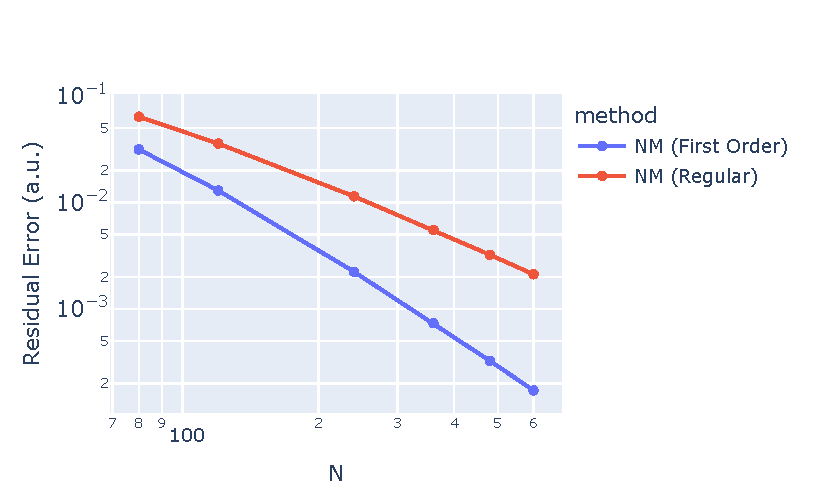
\includegraphics[width=\linewidth]{plots/first_order/residual_error.eps}
        \caption{השגיאה השיורית עבור תיקון מסדר ראשון}
        \label{fig:first_oreder_residual_error}
    \end{minipage}
    \hfill
    \begin{minipage}[t]{0.45\textwidth}
        \vspace{-4cm}
        \centering
        \begin{tabular}{|c|c|c|}
\hline
$K$ & שיטת נומרוב (סדר ראשון) & שיטת נומרוב \\
\hline
80 & $-0.46857$ & $-0.436174$ \\
\hline
120 & $-0.487077$ & $-0.464306$ \\
\hline
240 & $-0.497767$ & $-0.4886$ \\
\hline
360 & $-0.499266$ & $-0.494497$ \\
\hline
480 & $-0.499674$ & $-0.496776$ \\
\hline
600 & $-0.499828$ & $-0.497886$ \\
\hline
\end{tabular}

        \captionof{table}{אנרגיית היסוד עבור ערכי K שונים בשיטת נומרוב עם תיקון מסדר ראשון.}
        \label{tab:first_order_ground_energy}
    \end{minipage}%
\end{figure}
קבוע ההתכנסות ממהתאמה הוא \input{results/first_order/q_nm_o1} לעומת $q = 1.5539$ ללא התיקון, כלומר יש שיפור משמעותי בקצב ההתכנסות.
